\documentclass{beamer}
\usetheme{CambridgeUS}
\usepackage{amsmath}
\usepackage{amssymb}
\usepackage{tikz}
\usetikzlibrary{arrows.meta, positioning}
\usepackage{cancel}
\usetikzlibrary{positioning}
\usepackage{subcaption}
\usepackage{booktabs}

\tikzset{
box/.style={
draw,
rectangle,
rounded corners,
align=left,
font=\small,
inner sep=4pt,
fill=green!15
}
}



\title{On Solving the Multiple Variable Gapped Longest Common Subsequence Problem}

\author{Marko Djukanović\inst{1,2, 6}  \and Nikola Balaban\inst{2}  \and
Christian Blum\inst{3}  \and 
Aleksandar Kartelj\inst{4}  \and
Sašo Džeroski\inst{5}  \and
Žiga Zebec\inst{6}
}

\institute{ $^1$University of Nova Gorica, Nova Gorica, Slovenia \\ 
$^2$Faculty of Natural Sciences and Mathematics, University of Banja Luka, Banja Luka, Bosnia and Herzegovina \\ 
$^3$Artificial Intelligence Research Institute (IIIA-CSIC), Barcelona, Spain \\ 
$^4$Faculty of Mathematics, University of Belgrade, Belgrade, Serbia \\
$^5$Jožef Stefan Institute, Ljubljana, Slovenia \ \\
$^6$Institute of Information Sciences (IZUM), Maribor, Slovenia \\ \vspace{0.3cm}

\footnotesize{-- \textcolor{blue}{Eurocast 2026: 20th International Conference on Computer Aided Systems Theory, February 23-27, 2026,  Las Palmas de Gran Canaria, Spain}--}
\centering

\includegraphics[width=90pt,height=50pt]{SMASH_CMYK-ENG-horizontal_on_white.pdf}~ \hfill
\includegraphics[width=80pt,height=50pt]{IFEEL\_1.png}~\hfill
\includegraphics[width=110pt,height=40pt]{CofundedbytheEU\_RGB\_NEG.png}
}

\begin{document}
\begin{frame}[plain]
    \maketitle
\end{frame}

\begin{frame}{Outline}
    
    \begin{itemize}
        \item Introduction \& Preliminaries \vspace{0.2cm}
        \item Problem Definition  \vspace{0.2cm}
        \item Graph state space  \vspace{0.2cm}
        \item Iterative multi-source Beam Search  \vspace{0.2cm}
        \item Experimental Evaluation
        \begin{itemize}
            \item General problem
            \item Special problem
        \end{itemize} \vspace{0.2cm}
        \item Conclusions
    \end{itemize}
\end{frame}

\begin{frame}{Introduction}
   \begin{itemize}
       \item Objects we deal with: sequences (strings) over finite alphabet 
       \begin{itemize}
       \item DNA/RNA over $\{\texttt{A}, \texttt{T}, \texttt{G}, \texttt{C/U}\}$
       \item Proteins over 20 (canonical) amino acids: $\{\texttt{A}, \texttt{C}, \texttt{D}, \texttt{E}, \texttt{P}, \texttt{Q} ...\}$ 
       \end{itemize} \vspace{0.3cm}
       \item Computational biology
       \begin{itemize}
          \item \textbf{One of central tasks:} sequence comparison, finding common motifs between sequences
          \item compare structurally but also semantically/functionality 
          \item sequence alignment problems 
       \end{itemize} \vspace{0.4cm}
       
       \item Subsequences: reveal structural similarities $\rightarrow$ \textcolor{blue}{\textbf{Longest commmon subsequence problem}} variants
   \end{itemize}
\end{frame}

\begin{frame}{Longest common subsequence problem (LCSP)}
    
    \begin{itemize}
      \item Basic problem in Computational biology
      \item Intensively solved over last 50 years
      \begin{itemize}
      \item theoretically as well as practically 
      \item Practically: many approximation algorothms, (meta-) heuristics, exact approaches, etc.
      \end{itemize}
    \end{itemize}
    
    \begin{definition}[LCSP]
        \textbf{Input}: Given a set of sequences $S=\{s_1, \ldots, s_m\}$ \\
        \textbf{Task}: Find a   subsequence $s$ which is \textcolor{blue}{common} for all sequences from $S$ of \textcolor{blue}{maximum} possible length. 
    \end{definition}
    \begin{example}
       Input: S=\{\texttt{\textcolor{red}{A}A\textcolor{red}{T}\textcolor{red}{T}G\textcolor{red}{C}}, \texttt{\textcolor{red}{A}\textcolor{red}{T}\textcolor{red}{T}A\textcolor{red}{C}}\} \\ 
       LCS solution: s=\textcolor{red}{ATTC}
    \end{example}
\end{frame}

\begin{frame}{Literature \& LCS Problem Variants }
Theoretically:
  \begin{itemize}
  \item When $m=2$ -- polynomially solvable (in $O(n^2)$): \textcolor{blue}{Dynamic programming}, Hunt-Schlimanski, ... 
  \item When $m$ arbitrary large -- $\mathcal{NP}$-hard:
   \begin{itemize}
   \item subject of interest within last 30 years: approximation approaches, meta-heuristics (ACO, \textcolor{blue}{Beam search}, ...), but also exact approaches (A$^*$, anytime approaches,...)
   \end{itemize}  
  \end{itemize}\vspace{0.3cm}
  
  Problem-related variants:
  \begin{itemize}
  		\item Arc-annotated LCS problem
 		 \item Constrained (restricted/imposed) LCS problem
  		\item Repetition-free, Longest filled LCS,...
  		\item \textbf{Gapped LCS problem}
  \end{itemize}
\end{frame}

\begin{frame}{The gaped LCS problem}
   \begin{definition}[A gap sequence]
       Given is a sequence $s$ and an assigned function 
       $G_s \colon \{1, \ldots, |s|\} \mapsto \mathbb{N}$. An ordered pair $(s, G_s)$ is called a \textbf{sequence with gaps}.
   \end{definition} \vspace{0.5cm}
   
   \begin{definition}[A gapped subsequence]
         Sequence $\tilde{s}$ is a gapped subsequence of $(s, G_s)$ iff 
         \begin{itemize}
             \item $\tilde{s}$ is a subsequence of $s$
             \item the gapped constraint $G_s$ is fulfilled w.r.t.\ \textit{positions of appearances} of letters of $\tilde{s}$ in $s$
         \begin{itemize}
             \item  suppose $i_1, \ldots, i_{|\tilde{s}|}$ are \textbf{positions of embedding} $\tilde{s}$ in $s$
             \item ($\forall$ $j=2, \ldots, |\tilde{s}|)\, i_{j} - i_{j-1} \leq G_{s}(i_{j})+1$ 
         \end{itemize}
       \end{itemize}
   \end{definition}
   
\end{frame}

\begin{frame}{Problem definition}

   \begin{example}
      $s=\texttt{AATTGC}$, $G_s(\cdot)=1$
      \begin{itemize}
         \item  $\tilde{s}=\texttt{ATG}$, the embedding: \textcolor{red}{A}A\textcolor{red}{T}T\textcolor{red}{G}C (\textcolor{blue}{valid} gapped subsequence)
         \item  $\tilde{s}=\texttt{ATG}$, the embedding: \textcolor{red}{A}A{T}\textcolor{red}{T}\textcolor{red}{G}C (\textcolor{blue}{invalid} gapped subsequence)
      \end{itemize}
   \end{example} \vspace{0.3cm}
    
   \begin{definition}[The multiple (variable) gapped LCS problem -- MVGLCSP]
        \textbf{Input}: Given is a set of gapped sequences $(s_1, G_{s_1}), \ldots, (s_m, G_{s_m})$. \\
        \textbf{Task}: Find the longest  subsequence $\tilde{s}$ so that 
        \begin{itemize}
            \item  $\tilde{s}$ is common subusequence of each $s_i$
            \item $\tilde{s}$ fulfills all gap constraints $G_{s_i}$  for each $i=1, \ldots, m$
        \end{itemize}
    \end{definition}
    \textbf{Note}: when $G_{s_i}=n$ (the length of longest sequence) $\Rightarrow$ VGLCSP = LCSP.
\end{frame}

\begin{frame}{Literature \& Motivation}
   
   \begin{itemize}
       \item  Peng and Yang (2012, 2014): studied the problem with $m=2$ (poly-version): \textbf{Three dynamic programming} approaches (basic and sparse, sparse + advanced data-structures)
       \item  Manea et al. (2024): Complexity bounds,  (parameterised) complexity analysis investigated
       \item NP-hard under arbitrary $m$ 
   \end{itemize} \vspace{0.3cm}
   
   Motivation:
   \begin{itemize}
       \item  \textbf{Genetics and molecular biology}: applications in DNA and protein analysis where variable structural distances between residues must be respected
       \item \textbf{Time-series analysis}: in settings where events are required to occur within specified temporal delays~(Lainscsek et al. (2015))
   \end{itemize}
   
\end{frame}

\begin{frame}{Methodology}
    \begin{itemize}
        \item Based on the significant extension of the state space graph formulation for LCS problem  (Djukanovic et al. (2020)) \vspace{0.3cm}
        \item Gap constraints: incorporated to cut-off the invalid extensions (edges) among the LCS extensions immediately \vspace{0.3cm}
        \item Reach-ability of all extensions is an issue (\textbf{many root nodes} in the state graph, possibly separated subgraphs)
    \end{itemize}
    
\end{frame}


\begin{frame}{Root-based state graph formulation: rough idea}
  
  \begin{itemize}
      \item Each \textbf{state} $v=(p^L, l^v)$: one or more feasible partial solutions characterized by a vector of positions $p^L$ referring to relevant suffixes of input sequences to  further expand these sols, and by the current subsequence length $l^v$ \vspace{0.3cm}
      \item \textbf{Node expansion} of $v$: extend partial solutions feasibly by one letter  (concatenation) in all possible ways (like in LCS case),  respecting gap constraints \vspace{0.3cm}
      \item \textbf{Non-expandable nodes}: complete solutions 
  \end{itemize} \vspace{0.5cm}
  
  \fbox{\textcolor{red}{\textbf{Crucial: selection of position $r$ for root node 
   (corr.\ to empty part.\ sol.)}}} $\Rightarrow$ possibly \textbf{(exponentially) many root nodes}. \\ State graphs space induced by root node $(r, 0)$ we denote by \emph{Space(r)}.
\end{frame}

\begin{frame}{Root-based state graph formulation: example with the match $r=(1, 1)$ (obviously a valid root node)}
   
   % U nekom delu LaTeX dokumenta:
   \begin{figure}[h!]
   \centering
   \scalebox{0.4}{
   
   
   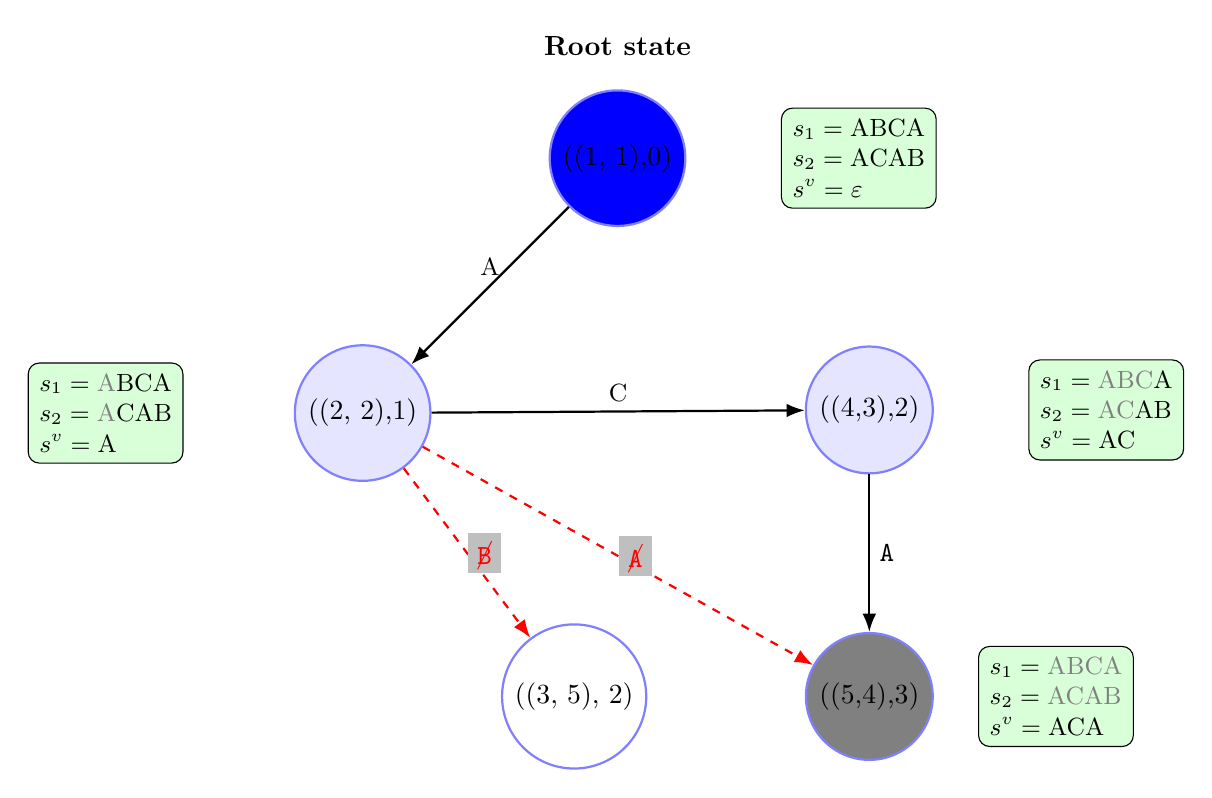
\begin{tikzpicture}[
   state/.style={circle, draw=blue!50, fill=blue!10, thick, minimum size=8mm},
   edge/.style={-Latex, thick},
   node distance=2cm and 2cm
   ]
   
   % Čvorovi
   \node[state, fill=blue] (s0) {((1, 1),0)};
   \node[state, below left=of s0] (s1) {((2, 2),1)};
   \node[state, below right=of s0] (s2) {((4,3),2)};
   %\node[state, below=of s2] (s3) {(4,3)};
   \node[state, below=of s2, fill=gray] (s4) {((5,4),3)}; % krajnje, ali ne koristi se ovde
   \node[state, left=of s4, fill=white] (s5) {((3, 5), 2)}; % krajnje, ali ne koristi se ovde
   
   % Right of root ((1,1),0)
   \node[box, right=12mm of s0] (b0) {
   $s_1=\text{{A}BCA}$\\
   $s_2=\text{{A}CAB}$\\
   $s^v=\varepsilon$
   };
   
   % Left of ((2,2),1)
   \node[box, left=14mm of s1] (b1) {
   $s_1=\text{\textcolor{gray}{A}BCA}$\\
   $s_2=\text{\textcolor{gray}{A}CAB}$\\
   $s^v=\text{A}$
   };
   
   % Right of ((4,3),2)
   \node[box, right=12mm of s2] (b2) {
   $s_1=\text{\textcolor{gray}{ABC}A}$\\
   $s_2=\text{\textcolor{gray}{AC}AB}$\\
   $s^v=\text{AC}$
   };
   
   % Right of ((5,4),3)
   \node[box, right=42mm of s5] (b3) {
   $s_1=\text{\textcolor{gray}{ABCA}}$\\
   $s_2=\text{\textcolor{gray}{ACAB}}$\\
   $s^v=\text{ACA}$
   };
   
 
   
   % Grane (samo validne poklapanja)
   \draw[edge] (s0) -- node[above] {\small A} (s1);
   %\draw[edge] (s0) -- node[above] {\small A} (s2);
   \draw[edge] (s1) -- node[above] {\small C} (s2);
   %\draw[edge] (s2) -- node[right] {\small A} (s3);
   %\draw[edge] (s3) -- node[right] {\texttt{A}} (s4);
   \draw[edge,  scale=2.2, dashed, red] (s1) -- node[right, fill=lightgray] {$\cancel{\texttt{B}}$} (s5);
   
    \draw[edge,  scale=2.2, dashed, red] (s1) -- node[right, fill=lightgray] {$\cancel{\texttt{A}}$} (s4);
   % Oznake
   \node[above=0.3cm of s0] {\textbf{Root state}};
   %\node[below=1.5cm of s3] {\small \textbf{Krajnje stanje}};
   \draw[edge] (s2) -- node[right] {\texttt{A}} (s4);
   
   \end{tikzpicture}}
   
   \caption{State space graph $Space(r=((1, 1), 0))$ for MVGLCSP between the sequences \texttt{ABCA} and  \texttt{ACAB}, assuming $G_1=G_2=1$.   % \fxnote{Add VGLCS example}
   }
   
   \label{fig:vgcs-grafstanja}
   \end{figure}
   
\end{frame}


\begin{frame}{An issue with the root-state-space formulation: example}

   \begin{itemize}
   \item The VGLCSP may exhibit multiple, potentially exponentially many, \emph{disconnected root components} in its complete state space.
   \item  If started from $(1, 1)$, it fails to reach    optimal solutions.     \end{itemize}
   \begin{example}
   		$
   		S = \{ s_1 = \texttt{ATGG\fbox{A}AA},\; s_2 = \texttt{ATCC\fbox{A}AA} \},
   		$
   		with gap constraints $G_{s_1} = G_{s_2} = 1$. In this instance, any state with position vector $\mathbf{p}^L = (5,5)$ cannot be reached  from the initial state $((1,1),0)$ by standard direct transitions. 

  \end{example} \vspace{0.5cm}
  
   \textbf{Consequence}: $((5, 5), 0) \not \in Space((1, 1))$  $\Rightarrow$  
   \textcolor{blue}{The optimal common subsequence \texttt{AAA} is unreachable.} %from the basic root $((1,1),0)$,  therefore missed by traditional search strategies.
   
\end{frame}

\begin{frame}{Iterative multi-source beam search (IMSBS) strategy}
      
      \begin{itemize}
      		\item \textbf{Full state space} of a VGLCSP instance: $\bigcup_{v \in \mathcal{R}} \mathrm{Space}(\mathbf{p}^{L, v})$, with $\mathcal{R}$ all root states  
      		\item Explicitly enumerating all root states computationally prohibitive (requiring $O(n^m)$ time) \vspace{0.3cm}
      		\item \textbf{IMSBS} (idea):
      		\begin{itemize}
      		    \item Based on \textbf{beam search}: limited breadth-first-search (BFS) strategy (for exploring \emph{Space(r)}), \textcolor{blue}{parameter $\beta$} controls the number of nodes to be further pursued
      		    
      		    \item dynamically explore multiple promising regions of the state space: move from one rooted subgraph to another one 
      		    \item \textbf{iteratively identifies and expands} a set of \textcolor{red}{promising} candidate root states
      		\end{itemize}
      \end{itemize}  
\end{frame}

\begin{frame}{Components and characteristics of IMSBS}
     
     
     \begin{itemize}
     	\item $\mathcal{R}$: a global set of root-node candidates, dynamically updated over iterations
     	\item \textbf{Beam search} (backward): not all candidate nodes from $\mathcal{R}$ are root nodes
     	\begin{itemize}
     		\item \textcolor{blue}{\textbf{refine}} them by performing the \textcolor{blue}{\textbf{backward}} approximate passes from candidate-root nodes to effectively reach distant (real) and promising root node in the state space
     	\end{itemize}
     	\item \textcolor{blue}{\textbf{Beam search}} (forward): \textcolor{red}{intensification} in the chosen root-space \emph{Space(p)}: seek for high-quality (complete) solutions in the corresponding search sub-regions
     	\item \textcolor{red}{diversification}:  during each BS (forward), the complete nodes  are expanded in all possible ways (gaps ignored) to generate candidates for roots (distant from the current region)
     \end{itemize}

\end{frame}

\begin{frame}{Working example}
	%start from the empty source node (0, 0), generating initial (proven) root nodes first -- for each a \in \Sigma => the first occurances of letter a as position p^{L, a} ...   
	 TODO: draw some plots regarding the workflow of the approach
	 
 
\end{frame}

\begin{frame}{The core advantages of the IMSBS approach}
 
     \begin{itemize}
     	\item Balance between complete beam search execution (local exploration of promising paths) and the generation of new source nodes (\textbf{global coverage} of the search space)
     	\item Preventing from direct suboptimal solutions reduced by executing backward beam search procedure (\textbf{refinement})
     \end{itemize}
      
\end{frame}

\begin{frame}{Heuristic guidances in BS}
    
    Three LCS heuristic guidances used:
        \begin{itemize}
       	    \item  \textit{``Look-ahead'' for the remaining length:}
    	    \begin{equation}
    		    \textrm{UB}_1(\mathbf{v}) = l^v + \min_{i = 1, \ldots, m} \left( |s_i| - p_i^v + 1 \right)
        	\end{equation}
    	  	\item  \textit{Character Frequency Alignment:}
    	   \begin{equation}
    	   	\textrm{UB}_2(\mathbf{v}) =  l^v + \sum_{\sigma \in \Sigma} 
    	   	\min \underbrace{\left( |s_1[p_1^v, |s_1|]|_{\sigma}, \ldots, |s_m[p_m^v, |s_m|]|_{\sigma} \right)}_{\text{remaining valid suffixes}}
    	   \end{equation}
    	   \item \textit{A probability-based heuristic} guidance $h_{prob}$: by the pre-processed matrices of probabilities (Mousavi and Tabataba~(2012)). These probabilities approximate the probability for the event that a sequence $s$ of length $k$ is a subsequence of a (random) sequence of length $n$ %over an alphabet $\Sigma$.
    \end{itemize}
\end{frame}

\begin{frame}{Experimental Evaluation: arbitrary large $m$-case}
	
	\begin{itemize}
		\item \textsc{Bs}: a baseline beam search approach, allowing \textbf{a single iteration} of IMSBS (utilizing a huge $\beta$)
		
		\item \textsc{Imsbs-greedy}: a variant of IMSBS with a fixed \textbf{beam-width parameter} \( \beta = 1 \) for the forward BS. This configuration highlights the impact of performing a larger number of beam search iterations on the overall performance of \textsc{Imsbs}
		\item \textsc{Imsbs}: a tuned version;  configured to use an average runtime comparable to that of \textsc{Bs}
	\end{itemize}
	
\end{frame}

\begin{frame}{Benchmark set \textsc{Random}}
	 
	 For each combination of instance parameters
	 \begin{itemize}
	 	  \item  $n \in \{50, 100, 200, 500\}$
	 	  \item $m \in \{2, 3, 5, 10\}$
	 	  \item $|\Sigma| \in \{2, 4\}$
	 \end{itemize} 
	 
	 10 random problem instances are generated (sequences uniformly at random). \\ \vspace{0.3cm}
	 
	 The gap constraints: generated such that $G_{s_i}(j) \in \mathcal{U}(\{ \lfloor 0.5 \cdot |\Sigma| \rfloor, \ldots, \lfloor 1.5 \cdot |\Sigma| \rfloor \})$.   \\ \vspace{0.7cm}
	 
	 $\Longrightarrow$ A total of \textcolor{red}{\textbf{320 problem instances}} is generated.
	 
\end{frame}

\begin{frame}{Parameter tuning of IMSBS}
	We fixed:
	\begin{itemize}
		\item \textsc{Bs}: $\beta=10$, and UB for the backwards BS (efficient)
		\item Candidate root nodes from $\mathcal{R}$ ordered by $UB$ (decreasingly)
		\item At each iteration, 10 best nodes from $\mathcal{R}$ taken
	\end{itemize} \vspace{0.3cm}
	
	Tuned parameters:
	\begin{itemize}
		\item $\beta$ (in BS-forward)
		\item Heuristic guidance in BS-forward
		\begin{itemize}
			\item $\{\text{UB}_1, \text{UB}_2, h\}$
		\end{itemize}
	\end{itemize}
	
	
\end{frame}

\begin{frame}{$\textsc{Bs}$: influence of $\beta$ and heuristic guidances}
	
	   \begin{figure}[!ht]
	  	\centering
	  	\begin{subfigure}[t]{0.48\textwidth}
	  		\centering
	  		\includegraphics[width=\linewidth, height=120pt]{figures/bs_tuning_quality.png}
	  		\caption{Avg. quality over all instances from the \textsc{Random} benchmark suite.}
	  		\label{fig:tune_bs}
	  	\end{subfigure}
	  	~
	  	\begin{subfigure}[t]{0.48\textwidth}
	  		\centering
	  		\includegraphics[width=\linewidth, height=120pt]{figures/bs_tuning_time.png}
	  		\caption{Avg. runtime over all instances from the \textsc{Random} benchmark suite.}
	  		\label{fig:tune_bs_time}
	  	\end{subfigure}
	  	\caption{Beam search tuning results on the \textsc{Random} benchmark suite.}
	  	\label{fig:bs_tuning}
	  \end{figure}
	  
	  $\Longrightarrow \beta = 10,000$ and $h = h_{\text{prob}}$
\end{frame}

\begin{frame}{Parameter tuning of \textsc{Imsbs}}
	
	 \begin{figure}[!h]
		\centering
		\begin{minipage}{0.48\textwidth}
			\centering
			\includegraphics[width=\linewidth]{figures/imsbs_tuning.png}
			\caption*{(a) Avg. quality for different IMSBS settings over all instances from the \textsc{Random} benchmark suite.}
			\label{fig:tune_imsbs}
		\end{minipage}
		~
		\begin{minipage}{0.48\textwidth}
			\centering
			\includegraphics[width=\linewidth]{figures/imsbs_tuning_time.png}
			\caption*{(b) Avg. runtime for different IMSBS settings over all instances from the \textsc{Random} benchmark suite.}
			\label{fig:tune_imsbs_time}
		\end{minipage}
		\caption{IMSBS parameter tuning results on the \textsc{Random} benchmark suite.}
		\label{fig:imsbs_tuning}
	\end{figure}
	
	$\Longrightarrow \textcolor{red}{h = \textrm{UB}_2}$ and $\textcolor{red}{\beta = 500}$.\\ \vspace{0.3cm}
	\textsc{Imsbs-Greedy}:  $\beta=1$, $imsbs\_iter=10,000$ (comparable avg. runtime to \textsc{Imsbs})
\end{frame}

\begin{frame}{Numerical results}
   
       
   
   \begin{table}[H]
   	%\caption{Numerical results on the \textsc{Random} benchmark suite. }\label{tab:numerical_results_general_m}
   	\centering
   	\scalebox{0.4}{
   		\begin{tabular}{lll|rr|rr|rr}
   			\hline
   			\multicolumn{3}{c}{Inst.} & \multicolumn{2}{c}{\textsc{Bs}} & \multicolumn{2}{c}{\textsc{Imsbs-Greedy}} & \multicolumn{2}{c}{\textsc{Imsbs}} \\
   			\cmidrule(lrr){1-3} \cmidrule(lr){4-5} \cmidrule(lr){6-7} \cmidrule(lr){8-9} \\ 
   			$m$ & $n$ & $|\Sigma|$ & $\overline{obj}$ & $\overline{t}[s]$ & $\overline{obj}$ & $\overline{t}[s]$ & $\overline{obj}$ & $\overline{t}[s]$ \\
   			\hline
   			\midrule
   			2 &       50 &         2 &            33.6 &         0.02 &                     33.1 &                  0.00 &         \textbf{37.7} &      0.06 \\
   			2 &       50 &         4 &            30.1 &         0.98 &                     27.7 &                  0.00 &         \textbf{30.1} &      0.16 \\
   			2 &      100 &         2 &            48.9 &         2.07 &                     64.5 &                  0.01 &         \textbf{72.8} &      0.94 \\
   			2 &      100 &         4 &            \textbf{62.1} &        11.19 &                     56.9 &                  0.01 &         61.6 &      0.91 \\
   			2 &      200 &         2 &            99.1 &        18.56 &                     95.5 &                  0.02 &        \textbf{136.4} &      6.21 \\
   			2 &      200 &         4 &           120.5 &        38.15 &                    116.1 &                  0.05 &        \textbf{124.9} &      6.58 \\
   			2 &      500 &         2 &            65.3 &        23.27 &                    153.6 &                  0.07 &        \textbf{265.7} &    119.75 \\
   			2 &      500 &         4 &           214.6 &       163.69 &                    227.7 &                  0.12 &        \textbf{294.4} &     60.49 \\ \hline
   			3 &       50 &         2 &            17.5 &         0.03 &                     27.2 &                  0.00 &         \textbf{31.2} &      0.14 \\
   			3 &       50 &         4 &            21.7 &         0.18 &                     21.5 &                  0.00 &         \textbf{22.9} &      0.19 \\
   			3 &      100 &         2 &            19.7 &         0.06 &                     41.8 &                  0.01 &         \textbf{58.5} &      3.15 \\
   			3 &      100 &         4 &            34.1 &         2.35 &                     43.4 &                  0.03 &         \textbf{48.4} &      5.58 \\
   			3 &      200 &         2 &            15.2 &         0.16 &                     63.6 &                  0.02 &         \textbf{90.0} &     22.48 \\
   			3 &      200 &         4 &            85.3 &        23.45 &                     77.2 &                  0.08 &         \textbf{97.1} &     72.25 \\
   			3 &      500 &         2 &            12.6 &         0.10 &                     69.9 &                  0.07 &        \textbf{102.9} &     53.56 \\
   			3 &      500 &         4 &            90.7 &        86.35 &                    104.2 &                  0.29 &        \textbf{187.7} &    412.27 \\ \hline
   			5 &       50 &         2 &             4.8 &         0.00 &                     14.9 &                  0.00 &         \textbf{20.0} &      0.36 \\
   			5 &       50 &         4 &             8.9 &         0.01 &                     13.6 &                  0.06 &         \textbf{15.3} &      0.79 \\
   			5 &      100 &         2 &             6.3 &         0.01 &                     17.7 &                  0.01 &         \textbf{22.4} &      0.57 \\
   			5 &      100 &         4 &             5.3 &         0.01 &                     \textbf{23.2} &                 10.85 &         22.1 &      1.44 \\
   			5 &      200 &         2 &             5.3 &         0.01 &                     21.6 &                  0.03 &         \textbf{26.6} &      1.07 \\
   			5 &      200 &         4 &             6.4 &         0.02 &                     \textbf{32.5} &                604.11 &         {25.7} &      2.10 \\
   			5 &      500 &         2 &             5.9 &         0.10 &                     25.5 &                  0.14 &         \textbf{27.9} &      3.22 \\
   			5 &      500 &         4 &             6.8 &         0.10 &                     \textbf{43.6} &               1341.25 &         26.9 &      3.52 \\ \hline
   			10 &       50 &         2 &             1.7 &         0.00 &                      8.8 &                  2.28 &          \textbf{9.1} &      0.47 \\ 
   			10 &       50 &         4 &             1.9 &         0.00 &                      \textbf{7.0} &                508.36 &          6.1 &      1.46 \\
   			10 &      100 &         2 &             1.1 &         0.00 &                     \textbf{14.0} &               1421.10 &          8.6 &      0.54 \\
   			10 &      100 &         4 &             2.2 &         0.01 &                      \textbf{8.9} &               1800.45 &          {6.3} &      1.51 \\
   			10 &      200 &         2 &             2.5 &         0.01 &                     \textbf{13.2} &               1710.49 &         10.3 &      0.77 \\
   			10 &      200 &         4 &             2.2 &         0.02 &                      \textbf{7.9} &               1800.54 &          6.1 &      1.74 \\
   			10 &      500 &         2 &             1.8 &         0.08 &                     \textbf{13.8} &               1611.70 &          {9.5} &      1.53 \\
   			10 &      500 &         4 &             1.9 &         0.09 &                      \textbf{8.2} &               1800.46 &          6.1 &      2.37 \\
   			\hline \hline
   			\textbf{Avg.} &  &  &  32.38 & 10.97 & 46.82 & 394.14 &  \textbf{59.73} & 24.63  \\ \hline \hline
   	\end{tabular}}
   \end{table}
   
   
\end{frame}

\begin{frame}{Numerical results for $m=2$ case}
	    
	    \begin{itemize}
	 	    \item \textsc{Dp}: the basic dynamic programming algorithm
	 	    \item \textsc{Dp}-1: an advanced dynamic programming approach that uses Incremental Suffix Maximum Queries (ISMQ) with \texttt{Col} and \texttt{All} matrices to accelerate the basic DP algorithm
	 	    \item \textsc{Dp}-2: an enhanced dynamic programming algorithm that handles ISMQ using a \textit{dequeue} data structure for further speedup
	 	    \item \textsc{Ilp}: an integer linear programming method \textbf{proposed in this work}, motivated by the ILP model for LCS problems
	 \end{itemize} \vspace{0.5cm}
\textcolor{blue}{\textbf{The first known empirical comparison for the $m=2$} (80 instances).}
\end{frame}

\begin{frame}{Experimental evaluation}
	 
	 \begin{table}[H]
	 	\caption{Results on the \textsc{Random} benchmark set for $m=2$: the exact approaches from the literature.}\label{tab:results-2d-literature}
	 	\centering
	 	\scalebox{0.7}{
	 		\begin{tabular}{lll|lr|rr|rr|rr}
	 			\hline
	 			\multicolumn{3}{c}{Inst.} & \multicolumn{2}{c}{\textsc{Dp}}  &
	 			\multicolumn{2}{c}{\textsc{Dp-1}} & \multicolumn{2}{c}{\textsc{Dp-2}} & 
	 			\multicolumn{2}{c}{\textsc{Ilp}}  \\
	 			\cmidrule(lrr){1-3} \cmidrule(lr){4-5}
	 			\cmidrule(lr){6-7} \cmidrule(lr){8-9}
	 			\cmidrule(lr){10-11} 	\\ 
	 			$m$ & $n$ & $|\Sigma|$ & $\overline{obj}$ & $\overline{t}[s]$ & $\overline{obj}$  & $\overline{t}[s]$ &$\overline{obj}$  & $\overline{t}[s]$ & $\overline{obj}$  & $\overline{t}[s]$ \\
	 			\hline
	 			2 &   50 &         2 &              38.1 &          0.01 & 38.1 &          \textbf{0.01} &              38.1 &          0.01  & 38.1 & 168.3 \\
	 			2 &   50 &         4 &              30.3 &          \textbf{0.01} &              30.3 &          0.02 &              30.3 &          0.02 & 30.3  & 28.0 \\ \hline
	 			2 &  100 &         2 &              77.4 &          0.1 &              77.4 &          \textbf{0.03} &              77.4 &          0.05 & -- & -- \\
	 			2 &  100 &         4 &              62.3 &          0.07 &              62.3 &         \textbf{0.06} &              62.3 &          0.09 & 0.00 & 1800.0 \\ \hline
	 			
	 			2 &  200 &         2 &             156.4 &          0.75 &             156.4 &          \textbf{0.13} &             156.4 &          0.16  & -- & -- \\
	 			2 &  200 &         4 &             127.2 &          0.59 &             127.2 &          \textbf{0.25} &             127.2 &          0.32  & -- & -- \\ \hline
	 			
	 			2 &  500 &         2 &             395.9 &         13.57 &             395.9 &          \textbf{0.84}  &             395.9 &          1.05 & -- & -- \\
	 			2 &  500 &         4 &             317.2 &         10.18 &             317.2 &          \textbf{1.70} & 317.2 &  2.1 & -- &-- \\    
	 			\hline \hline
	 	\end{tabular}}
	 	
	 \end{table} 
	 
	 
	 
	 
\end{frame}

\begin{frame}{The $m=2$ case: heuristic performance vs. optimal solution }
	
	  \begin{figure}[htbp]
		\centering
		\begin{minipage}{0.48\textwidth}
			\includegraphics[width=\linewidth]{figures/bs_imsbs_imbs_greedy_vs_dp_quality_distribution.png} 
			\caption*{(a) Relative solution quality percentage distribution for each heuristic approach with respect to the optimal solutions.} 
		\end{minipage}
		\hfill
		\begin{minipage}{0.48\textwidth}
			\centering
			\includegraphics[width=\linewidth]{figures/bs_imsbs_imsbs_greedy_vs_dp_quality.png}
			\caption*{(b) Relative solution quality achieved by the heuristic approaches compared to the optimal solutions.}
		\end{minipage}
		%\caption{Number of instances for which \textsc{Bs} and \textsc{Imsbs} achieve a specific ratio of the obtained (approximate) solution quality to the known optimal solution for $m=2$.}
		%\label{fig:optimal-vs-heuristic}
	\end{figure}
	
	
\end{frame}

\begin{frame}{Conclusions and Future Work}
	
	\begin{itemize}
		\item Proposed a general heuristic approach to solve the VGLCS problem with arbitrary input strings 
		\item IMSBS designed: combines Beam search (backward and forward manner) in an iterative way while producing promising source nodes as candidates of further iterations
		\item Balancing intensification and diversification 
		\item Empirical studies conducted for the first time on synthetic instances: the tuned IMSBS clearly wins over the baseline Beam search approach  
	\end{itemize}    \vspace{0.5cm}
	
\textbf{Future work:}
	\begin{itemize}
		\item Real-world instance-case scenario
		\item Data-driven heuristic involving locl and global instance features (NN-based)
	\end{itemize}
\end{frame}

\begin{frame}
	
	\centering
	\Large{\textcolor{blue}{\textbf{Thank you for your attention!}}}
	
\end{frame}


\end{document}
